\documentclass[10pt]{article}
\usepackage{graphicx} % Required for inserting images
\usepackage{amsmath}
\usepackage{amssymb}
\usepackage[margin=0.75in]{geometry}
\usepackage{algorithm2e}
\usepackage{fancyhdr}
\usepackage{caption}

%############################ SETTINGS
\RestyleAlgo{ruled}
% \pagestyle{fancy} % Apply headers to all pages
% \fancyhf{} % Clear all header and footer definitions
% % \fancyhead[L]{\small Adaptive Superpixel Cuts for Hyperspectral Images}
% % \fancyhead[R]{\small \thepage}
\DeclareMathOperator*{\argmax}{arg\,max}
\DeclareMathOperator*{\argmin}{arg\,min \;\;}
\DeclareMathOperator*{\diag}{diag}
\DeclareMathOperator*{\proj}{\text{proj}}
\DeclareMathOperator*{\cut}{\text{cut}}
\DeclareMathOperator*{\ncut}{\text{ncut}}
\DeclareMathOperator*{\assoc}{\text{assoc}}
% #############################################
% 
% 
% 
% 
% 
% #############################################
\title{Adaptive Superpixel Cuts for Hyperspectral Images}
\author{Aleksandar Popovic}
\date{February 2024}

\begin{document}

\maketitle

\begin{abstract}
    Blind segmentation in hyperspectral images is a challenging problem. Many traditional methods suffer from poor identification of materials and expensive computational costs, which can be partially eased by trading the accuracy with efficiency.

    In this paper, we propose a novel graph-based algorithm for segmentation in hyperspectral images. Utilizing the fact that pixels in a local region are likely to have similar spectral features, a pre-clustering algorithm is used to extract the homogenous regions, called superpixels. After extracting the superpixels, a weighted graph is constructed with the weights representing both the spectral similarity and spatial distance between each superpixel and its neighbors. The normalized graph cuts algorithm is then used to perform an initial segmentation of the image. To effectively extract the material information in the superpixels, the mean spectra in each segment is used to estimate the abundance of each endmember in each superpixel using a graph regularized hyperspectral unmixing algorithm. The resulting abundance information is used as a supportive feature, which when combined with the spectral features, form a new spectral feature vector for each superpixel. Using this new feature vector, the weighted graph is once again constructed and the normalized cuts algorithm is applied, resulting in a final segmentation of the image.

    Experiments on a real hyperspectral datasets illustrate great potential of the proposed method in terms of accuracy and efficiency.
\end{abstract}

\clearpage
% #############################################
% 
% 
% 
% 
% 
% #############################################
\tableofcontents

\clearpage
% #############################################
% 
% 
% 
% 
% 
% #############################################
\section{Introduction}

\subsection{Motivations}
\subsection{Applications to Biomedical Imaging}
\subsection{Hyperspectral Data}

\clearpage
% #############################################
% 
% 
% 
% 
% 
% #############################################
\section{Background} \label{Background}
% In hyperspectral imaging, near contiguous narrow band spectral information is measured for each spatial pixel of an image collected over a scene. Spectral information can be quantified by multiple measures. Traditionally, spectral radiance, being the energy emitted or reflected by a surface over a large number of spectral wavelengths, has been the measure of choice for physical applications. Utilizing this spectral information, physical and chemical properies of materials can be deduced and insights can be made about the overall composition of the images, resulting in applications across various fields.
Analysis in hyperspectral images has traditionally been a computationally expensive and difficult task due to algorithms scaling in both the spatial and spectral resolution of the images. This section will focus on building a relevant background for common preclustering, abundance estimation, and segmentation techniques from the perspective of imaging that will be later be adapted for use in the proposed algorithm. 


% \subsection{Hyperspectral Imaging: Basics} \label{Basics}
% In hyperspectral imaging, near contiguous narrow band spectral information is measured for each spatial pixel of an image collected over a scene. Spectral information can be quantified by multiple measures. Traditionally, spectral radiance, being the energy emitted or reflected by a surface over a large number of spectral wavelengths, has been the measure of choice for physical applications. Utilizing this spectral information, physical and chemical properies of materials can be deduced and insights can be made about the overall composition of the images, resulting in applications across various fields.

Analysis in hyperspectral images has traditionally been a computationally expensive and difficult task due to algorithms scaling in both the spatial and spectral resolution of the images. This section will focus on building a relevant background for common preclustering, abundance estimation, and segmentation techniques that are common in hyperspectral image analysis.


\subsection{The Hyperspectral Cube} \label{Cube}
In traditional, RGB based imaging systems, an image can be represented by a 3-dimensional tensor of shape $(n_x, n_y, 3)$, where the last dimension corresponds to the color channel the image was captured in. From a mathematical point of view, a hyperspectral image, denoted by $\mathbf{X}$, is a tensor of shape $(n_x, n_y, n_\lambda)$ with nonnegative entries. Each pixel in the tensor is represented using a vector $\mathbf{x} \in \mathbb{R}_+^{n_\lambda}$. From a physical point of view, the first two dimensions in $\mathbf{X}$ represent the spatial coordinates  of the pixels, while the last dimension represents the specific wavelength band the spectral intensity, reflectance or transmittance measurements were taken at.

The tensor $\mathbf{X}$ can be transformed into a two-dimensional matrix of shape $(n_p, n_\lambda)$, denoted $\mathbf{X}_f$, where $n_p = n_x n_y$ is the total number of pixels in the image, with each column representing the pixel at index $(i,j)$ in $\mathbf{X}$, arranged across the first spectral dimension, then the second. Formally, $$
\mathbf{X}_f = \left[ \mathbf{x}_{(0,0)},  \cdots, \mathbf{x}_{(n_x,0)}, \cdots, \mathbf{x}_{(0,n_y)}, \cdots, \mathbf{x}_{(n_x, n_y)} \right].
$$



\clearpage
\subsection{Superpixel Generation} \label{Superpixel}
In \ref{SLIC}, the SLIC algorithm was introduced, aiming to perceptually group pixels into locally homogeneous groups called superpixels. While the SLIC algorithm was originally developed for use in the CIELAB colorspace, a similar methodology can be applied towards the hyperspectral space. The main change when trasitioning to the hyperspectral domain requires the consideration of all the spectral features.

With the preprocessed hyperspectral image $\hat{\mathbf{X}}$, each pixel is represented by the vector $\hat{\mathbf{x}}_{(i,j)} = [\hat{x}_1, \hat{x}_2, \dots, \hat{x}_{n_\lambda}]$. Then, taking as an input the number of superpixels $n_s$, superpixel centroids $\mathbf{c}_n = [c_1, c_2, \dots, c_{n_\lambda}]$ where $n = 1,\dots, n_s$ are created at regular grid intervals $S = \sqrt{n_s/n_p}$ across the image. The initial centroids are moved to the lowest gradient position in a $3 \times 3$ spatial neighborhood where the image gradient is now calculated using the original hyperspectral features instead of the CIELAB features: 
\begin{equation}
    \label{eq:slic-gradient-2}
    \mathbb{G}(i,j) = \|\hat{\mathbf{x}}_{(i+1,j)} - \hat{\mathbf{x}}_{(i-1,j)} \|_2^2 + \|\hat{\mathbf{x}}_{(i,j+1)} - \hat{\mathbf{x}}_{(i,j-1)} \|_2^2
\end{equation}

Following the original formulation of the SLIC algorithm, a modified distance measure is proposed to enforce color similarity and spatial extent within the superpixels. Using the same parameter $m$ to control the compactness and shape of the superpixels, the modified distance between a pixel $\hat{\mathbf{x}}$ and cluster $\mathbf{c}_n$ is now calculated as $L_2$ difference between the spectral features plus a scaled version of the spatial euclidean distance between the pixel and the cluster center:
\begin{equation}
    \label{eq:slic-cielab-distance-hsi}
    \mathbb{D}(\hat{\mathbf{x}}, \mathbf{c}_n) = \|\hat{\mathbf{x}} - \mathbf{c}_n\|_2^2 + \frac{m}{S}d_{\text{spatial}}(\hat{\mathbf{x}}, \mathbf{c}_n)^2
\end{equation}

Each pixel is associated with the nearest cluster $\mathbf{c}_n$ whose search area overlaps the pixel. After all pixels are associated with a cluster, a new cluster center is computed as the average vector of all the pixels belonging to the cluster. This is repeated for a set number of iterations. In the hyperspectral version of the SLIC algorithm, the option of relabelling disjoint segments is not performed, instead opting for higher selection of the $m$ and $n_s$ parameters to avoid disjoint segments all together. Once the algorithm is completed, the final superpixeled image is given by arranging the feature vectors into columns of the matrix $\mathbf{C} = [\mathbf{c}_1 \; | \;\mathbf{c}_2 \;| \;\dots \;|\; \mathbf{c}_{n_s}] \in \mathbb{R}^{n_\lambda \times n_s}$. 

\begin{algorithm}[H]
    \label{HSI SLIC}
    \caption{Hyperspectral SLIC Algorithm}
    \textbf{Input}:\\
    \quad  Preprocessed Hyperspectral Image $\hat{\mathbf{X}}$\\
    \quad $m > 0$, $n_s > 0$, $k_{\text{max}}$\\

    \textbf{Initialize:} $\mathbf{c}_n = [c_1, c_2, \cdots, c_{n_\lambda}]$ where $n = 1, \cdots, n_s$ by sampling pixels at regular grid intervals $S$. Perturb cluster centers to lowest gradient position in a $3 \times 3$ neighborhood according to \eqref{eq:slic-gradient-2}. \\
    
    \For{$k = 1$ \KwTo $k_{\text{max}}$}{ 
        Assign best matching pixels from a $2S \times 2S$ neighborhood around clusters $\mathbf{c}_k$ according to \eqref{eq:slic-cielab-distance-hsi}.\\
         Compute new cluster centers according to average of all pixels belonging to cluster.
    }
    \textbf{Output}: Superpixeled Image Matrix $\mathbf{C}$
\end{algorithm}


In the hyperspectral domain, superpixels are slightly less adept at creating visually meaningful partitionings due to use of the raw hyperspectral spectra rather than a perceptual colorspace like CIELAB. To alleviate this, higher values of $m$ and $n_s$ are used to form more spatially compact regions akin to the ones formed in the original algorithm. Nonetheless, superpixels are valuable in allowing practioners to avoid having to consider the variation between individual pixels and instead consider the spectral and spatial variations between these new perceptual groupings of pixels. 
\subsubsection{Simple Linear Iterative Clustering} \label{SLIC}
In this section, we will introduce the Simple Linear Iterative Clustering (SLIC) algorithm. The algorithm is a special case of the k-means algorithm adapted to the task generating superpixels in a $5$-dimensional space, where the first $3$ dimensions correspond to the the pixel color vector in the CIELAB colorpsace. Formally, each pixel $\mathbf{x}_{(i,j)} = [x_l, x_a, x_b]$. 

Taking as an input the desired number of superpixels $n_s$, for an image with $n_p = n_x n_y$ pixels, each superpixel would be composed of approximately $n_s / n_p$ pixels. Assuming the superpixels lie on a grid, a superpixel centroid would occur at every grid interval $S = \sqrt{n_s/n_p}$. At the onset of the algorithm, a grid of $n_s$ superpixel centers $\mathbf{C}_n = [c_{l}, c_{a}, c_{b}]$ where $n = 1, \cdots, n_s$ are sampled across the image with regular grid intervals $S$. To avoid sampling noisy pixels, clusters are moved to the lowest gradient position in a $3 \times 3$ neighborhood where the image gradient is calcuated, using the original spectral vector $\mathbf{x}$ in the CIELAB color space as:
\begin{equation}
    \label{eq:slic-gradient}
    \mathbb{G}(i,j) = \|\mathbf{x}_{(i+1,j)} - \mathbf{x}_{(i-1,j)} \|^2 + \|\mathbf{x}_{(i,j+1)} - \mathbf{x}_{(i,j-1)} \|^2
\end{equation}

After initialization, a modified distance measure is proposed to enforce color similarity and spatial extent within the superpixels. Since the approximate area of each superpixel is $S^2$, it is assumed that pixels associated with a superpixel lie within a $2S \times 2S$ neighborhood of the superpixel centroid. Introducing the parameter $m$ to control the compactness and shape of the superpixels, the modified distance is then calculated as 
\begin{equation}
    \label{eq:slic-cielab-distance}
    \mathbb{D}(\mathbf{x}, \mathbf{c}_n) = \|\mathbf{x} - \mathbf{c}_n\|_2^2 + \frac{m}{S}d_{\text{spatial}}(\mathbf{x}, \mathbf{c}_n)^2
\end{equation}

Each pixel is the image is associated with the nearest cluster whose search area overlaps this pixel. After all pixels are associated with a cluster, a new center is computed as the average feature vector of all the pixels belonging to the cluster. This is repeated for a set number of iterations $k_\text{max}$. 

\begin{algorithm}[H]
    \caption{SLIC Superpixel Algorithm}
    \textbf{Input}: \\
    \quad CIELAB Image $\mathbf{X}$
    \quad  $m > 0$, $n_s > 0$, $k_{\text{max}} > 0$
    \\
    \textbf{Initialize:} $\mathbf{c}_n = [c_{l}, c_{a}, c_{b}, i, j]$ where $n = 1, \cdots, n_s$ by sampling pixels at regular grid intervals $S$. Perturb cluster centers to lowest gradient position in a $3 \times 3$ neighborhood according to \eqref{eq:slic-gradient} \\
    
    \For{$k = 1$ \KwTo $k_{\text{max}}$}{ 
        Assign best matching pixels from a $2S \times 2S$ neighborhood around clusters $C_k$ according to distance measure \eqref{eq:slic-cielab-distance}. \\
        Compute new cluster centers according to average vector of all pixels belonging to cluster.
    }
    \textbf{Output}: Superpixeled Image $\mathbf{X}_s = [\mathbf{c}_1, \mathbf{c}_2, \dots, \mathbf{c}_{n_s}]$
\end{algorithm}

The SLIC algorithm is shown to produce meaningful and noise-robust segments in traditional computer vision applications. This algorithm proves useful in Section \ref{Algorithm Superpixels} when adapted as a spatial preprocessing step in the hyperspectral domain.


\clearpage
\subsection{Hyperspectral Unmixing} \label{Unmixing Intro}
In hyperspectral imaging applications, spectral unmixing emphasizes estimating the relative abundance of a given representantive material, called an endmember, within each pixel.  Unmixing results often give more detailed information about the overall composition of a hyperspectral scene with a set of selected endmembers. This section will introduce the foundational knowledge behind unmixing and abundance estimation. 


\subsubsection{Linear Mixing Model}\label{LMM}
In reality, most pixels in a hyperspectral image capture a mixture of spectra reflected from various materials present within the spatial area, due to constraints with how large a spatial resolution can be acheived. The foundational model behind hyperspectral unmixing is the linear mixing model, which dictates that spectra of every pixel $\mathbf{x} \in \mathbb{R}_+^{n_\lambda}$ in a hyperspectral image is a linear combination of a set of $n_e$ spectra, $\mathbf{m} _1, \mathbf{m} _2, \cdots, \mathbf{m} _{n_e} \in \mathbb{R}_+^{n_\lambda}$, from pure representative materials, called endmembers, with weights $a_1, a_2, \cdots, a_{n_e} \in \mathbb{R}$. Denoting $\mathbf{M} = [\mathbf{m} _1 \;|\; \mathbf{m} _2 \;|\; \cdots \;|\; \mathbf{m} _{n_e}] \in \mathbb{R}_+^{n_\lambda \times n_e}$ and $\mathbf{a} = [a_1, a_2, \cdots ,a_{n_e}]^T \in \mathbb{R}^{n_e}$, the linear mixing model is formulated as follows:

\begin{equation}
    \label{lmm:model}
    \mathbf{x} = \mathbf{M} \mathbf{a} + \mathbf{\epsilon} 
\end{equation}

While this unconstrained model serves useful to unmixing an image, there is no direct physical interpretation to the weights in $\mathbf{a}$. Instead, we aim to estimate the physical proportion, called the abundance, of each endmember within each pixel by imposing two constraints on the entries in $\mathbf{a}$. The abundance nonnegativity constraint (ANC) requires that the entries in $\mathbf{a}$ must be greater than or equal to zero, while the abundance sum-to-one constraint (ASC) requires that the entries in $\mathbf{a}$ sum to $1$ (\cite{UNMIX}). Combining the two constraints, we have an extension of the linear mixing model

\begin{equation}
    \label{lmm:abund-lmm}
    \mathbf{x} = \mathbf{M} \mathbf{a} + \mathbf{\epsilon} \quad \text{ s.t } \mathbf{a} \in \mathbb{R}_+^{n_e} \text{ and } \|\mathbf{a}\|_1 = 1 
\end{equation}

The linear mixing model can be additionally be extended from a per pixel basis onto a collection of $n_p$ pixels $\mathbf{X} = [\mathbf{x}_1 \;|\; \mathbf{x}_2 \;|\; \cdots \;|\; \mathbf{x}_{n_p}] \in \mathbb{R}_ +^{n_\lambda \times n_p}$, with each pixel $\mathbf{x}_i$ having a corresponding abundance vector $\mathbf{a}_i$. Arranging the abundance vectors into an abundance matrix $\mathbf{A} = [\mathbf{a}_1 \;|\; \mathbf{a}_2 \;|\; \cdots \;|\; \mathbf{a}_{n_p} ] \in \mathbb{R}^{n_e \times n_p}$, we denote the ANC-ASC constraint using the set $ \Delta = \{ \mathbf{A} \in \mathbb{R}_+^{n_e \times n_p} \mid \mathbf{1}_{n_e}^T \mathbf{A} = \mathbf{1}_{n_p}\} $. The following natural extension of the linear mixing model to a collection of pixels will be the base for the following sections

\begin{equation}
    \label{lmm:abund-lmm-collection}
    \mathbf{X} = \mathbf{M} \mathbf{A} + \epsilon \quad \text{ s.t } \mathbf{A} \in \Delta
\end{equation}

The linear mixing model (\eqref{lmm:abund-lmm-collection}) is an simplistic model, which enforces a linear relationship between the spatial mixing of endmembers through assuming that pixels lie on a flat plane, as such, pixel measurements are dictated by how much each endmember is present. The model itself remains a efficient and powerful tool for extracting spectral information from a scene, even in modern analysis.
\subsubsection{Abundance Estimation}\label{AE}
Given the linear mixing model as formulated in Section \ref{LMM}, in traditional hyperspectral imaging tasks, both $\mathbf{M}$ and $\mathbf{A}$ are unknown. Often, researchers aim to estimate $\mathbf{M}$ first, as spectral signatures collected from endmembers in same scene under the same conditions will be almost identical. Notably, in the field of remote sensing, effort has been made to create a library of spectral signatures derived from common vegetation and minerals in land cover images, allowing focus to be made solely in estimating $\mathbf{A}$ [REF]. This section will cover the scenario where $\mathbf{M}$ is known and $\mathbf{A}$ is to be estimated. 

The task is referred to as abundance estimation and continues to be an active area of research, where the aim is to find $\mathbf{A}$ such that an error function $\mathcal{L}$ is minimized with respect to the reconstructed collections of pixels $\tilde{\mathbf{X}} = \mathbf{MA}$ and the original collection of pixels $\mathbf{X}$. Traditionally, we aim to minimize the least-square reconstruction error between the entries in $\tilde{\mathbf{X}}$ and $\mathbf{X}$

\begin{equation}
    \label{ae:fnorm}
    \mathcal{L}(\mathbf{X},\tilde{\mathbf{X}}) = \sum_{i=1}^{n_b} \sum_{j=1}^{n_p} \left(\mathbf{x}_{(i,j)} - \tilde{\mathbf{x}}_{(i,j)}\right)^2 = \|\tilde{\mathbf{X}} - \mathbf{X}\|_F^2.
\end{equation}

The least-squares reconstruction error can alternatively be written as the squared Frobenius norm, denoted as $\|\cdot\|_F^2$, of the difference between  $\tilde{\mathbf{X}}$ and $\mathbf{X}$. This choice of $\mathcal{L}$ is the straightforward approach as $\mathcal{L}$ is both convex and differentiable, with the additional properties that $\mathcal{L}(\tilde{\mathbf{X}},\mathbf{X}) = \mathcal{L}(\mathbf{X},\tilde{\mathbf{X}})$ and $ \mathcal{L}(\mathbf{X},\tilde{\mathbf{X}}) = \mathcal{L}(\mathbf{X}^T,\tilde{\mathbf{X}^T})$ [REF].

To incorporate the ANC-ASC constraint into the overall formulation of $\mathcal{L}$, the set $\Delta$ from Section \ref{LMM} proves useful. It is important to note that $\Delta$ is a convex set, meaning that for matrices $A, B \in \Delta$, for all $0 \leq \alpha \leq 1$, the matrix $C = \alpha A + (1- \alpha)B$ is also an element of $\Delta$. The inclusion of the constraints on $\mathbf{A}$ is facilitated using the piecewise function $\chi_S$ defined as follows

\begin{equation}
    \label{ae:indfunc}
    \chi_{S}(x) = 
            \begin{cases}
            0 &\text{if } x \in S \\
            \infty &\text{if } x \not \in S.
            \end{cases}
\end{equation}

Adding $\chi_\Delta$ in the formulation of $\mathcal{L}$ restricts the values $\mathbf{A}$ can take on to the set $\Delta$ while ensuring that the overall formulation still has a global minimum within $\Delta$. Additionally, a regularization term $J$ can be added to impose other constraints on the values in $\mathbf{A}$. Later sections operate on the assumption that $J$ is also convex. Formally, abudance estimation can be formualated as a convex optimization problem of the form

\begin{equation}
    \label{ae:ae-min-1}
    \mathbf{A} = \argmin_{\mathbf{A} \in \mathbb{R}^{n_e \times n_p}} \frac{1}{2}\|\mathbf{MA} - \mathbf{X}\|_F^2 + \chi_\Delta(\mathbf{A}) + J(\mathbf{A}).
\end{equation}

This problem has no closed form solution, relying on iterative methods or applying solvers like GUROBI [REF] or CVXOPT [REF] to solve the problem for individual pixels given the problem can be split pixelwise. The formulation of the abundance estimation allows for flexibility in choice of $\mathcal{L}$. There is particular interest in choosing $\mathcal{L}$ such that it is convex and differentiable, in order to apply gradient-based methods to estimate the abundance matrix, however there exist approaches that choose rely on divergence-based or non differentiable metrics [REF].

\clearpage
\subsection{Alternating Direction Method of Multipliers}\label{ADMM Intro}
Alternating Direction Method of Multipliers, or ADMM, introduced by Boyd et al. [REF] is a framework for solving convex optimization problems of the form:
\begin{equation}
    \label{admm:prob}
    \begin{aligned}
    &\text{minimize} \quad f(x) + g(z) \\
    &\text{subject to} \quad Ax + Bz = c
    \end{aligned}
\end{equation}
with variables $x \in \mathbb{R}^{n}$ and $z \in \mathbb{R}^{m}$, where $A \in \mathbb{R}^{p \times n}$, $B \in \mathbb{R}^{p \times m}$ and $c \in \mathbb{R}^{p}$. $f$ and $g$ are assumed to be convex. The aim of ADMM is to incorporate the decomposability of the dual ascent method into the superior convergence properties of method of multipliers. To allow for this, ADMM introduces the corresponding augmented Lagrangian $\mathcal{L}_{\mu}$ defined as:
\begin{equation}
    \label{admm:lagrangian}
    \mathcal{L}_{\mu}(x,z,y) = f(x) + g(z) + y^T(Ax + Bz - c) + \frac{\mu}{2} \|Ax + Bz - c\|_2^2
\end{equation}
where $\mu > 0$ is augmented lagrangian convergence parameter and $y \in \mathbb{R}^{p}$ is the corresponding dual variable. Scaling with $u  = \frac{1}{\mu} y $ gives the following equivalent definition: 
\begin{equation}
    \label{admm:lagrangian-real}
    \mathcal{L}_{\mu}(x,z,u) = f(x) + g(z) + \frac{\mu}{2} \|Ax + Bz - c + u\|_2^2.
\end{equation}

ADMM aims to minimize scaled form of $\mathcal{L}_{\mu}$ by alternating minimizations with respect to $x$, $y$, and $u$ by performing the following updates:

\begin{equation}
    \label{admm:updates}
    \begin{aligned}
        x^{(k+1)} &= \argmin_{x} \mathcal{L}_{\mu}(x,z^{(k)},u^{(k)})  \\
        z^{(k+1)} &= \argmin_{z} \mathcal{L}_{\mu}(x^{(k+1)},z,u^{(k)}) \\
        u^{(k+1)} &= u^{(k)} + Ax^{(k+1)} + Bz^{(k+1)} - c.
    \end{aligned} 
\end{equation}

Under mild conditions on $f$ and $g$, ADMM can be shown to provide guarenteed objective and residual convergence, independent on choice of $\mu$. For lax choices of $\mu$, the algorithm provides modest accuracy solutions in a relatively low number of iterations, favorable to tasks in statistical learning where parameter estimation often yields little improvement to results. The algorithm allows practioners to put focus on efficient implementations to the minimization problems for $x$ and $z$, and not on parameter tuning.


% \subsubsection{Abundance Estimation using ADMM}\label{Block ADMM}
%  In Section \ref{AE}, the abundance estimation problem for a collection of pixels $\mathbf{X}$ given the endmember spectra matrix $\mathbf{M}$ was known was stated as follows:

\begin{equation*}
    A = \argmin_{A \in \mathbb{R}^{n_e \times n_p}} \frac{1}{2}\|\mathbf{MA} - \mathbf{X}\|_F^2 + \chi_\Delta(\mathbf{A}) + J(\mathbf{A}).
\end{equation*}

The goal of this section is to demonstrate how this problem can be equivalently represented in a form where ADMM can directly be applied. The section itself operates under the assumption that $J$ is a convex function, for nonconvex choices of $J$, convergence is not guarenteed. The approach to transforming \eqref{ae:ae-min-1} is to first introduce matrices $\mathbf{U} \in \mathbb{R}^{n_e \times n_p}$, $\mathbf{V}_1 \in \mathbb{R}^{n_b \times n_p}$, $\mathbf{V}_2 \in \mathbb{R}^{n_e \times n_p}$, and $\mathbf{V}_{3} \in \mathbb{R}^{n_e \times n_p}$ and rewrite the problem into the equivalent form 
\begin{equation}
    \label{ae:equivalent-admm-1}
    \begin{aligned}
        \underset{\mathbf{U}, \mathbf{V}_1, \mathbf{V}_2, \mathbf{V}_2}{\textbf{minimize }} & \frac{1}{2} \|\mathbf{V}_1 - X \|_F^2 + \chi_{\Delta}(\mathbf{V}_2) + J(\mathbf{V}_3) 
        \\         
        \textbf{subject to } & \mathbf{V}_1 = \mathbf{MU} \\
        &\mathbf{V}_2 = \mathbf{U} \\
        &\mathbf{V}_{3} = \mathbf{U}.
   \end{aligned}
\end{equation}
Further rewriting the problem, the application of ADMM can clearly be seen:
\begin{equation}
    \label{ae:equivalent-admm-2}
    \begin{aligned}
        \underset{\mathbf{U},\mathbf{V}}{\textbf{minimize }} & g(\mathbf{V})
        \\         
        \textbf{subject to } & \mathbf{GU} + \mathbf{BV} = \mathbf{0}
   \end{aligned}
\end{equation}
where 
$
g(\mathbf{V}) = \frac{1}{2} \|\mathbf{V}_1 - X \|_F^2 + \chi_{\Delta}(\mathbf{V}_2) + J(\mathbf{V}_3) 
$, 
$$
\mathbf{V} = \begin{bmatrix}
\mathbf{V}_1 &  &   \\
 &\mathbf{V}_2&   \\
  &  & \mathbf{V}_3 \\
\end{bmatrix},
\quad
\mathbf{G} = 
\begin{bmatrix}
\mathbf{M}\\ 
\mathbf{I}\\ 
\mathbf{I}\\ 
\end{bmatrix},
\quad
\mathbf{B} = 
\begin{bmatrix}
-\mathbf{I} &  &  \\
  &-\mathbf{I}&  \\
&  & -\mathbf{I} \\
\end{bmatrix}.
$$

With parameter $\mu > 0$, the augmented lagrangian $\mathcal{L}_\mu$ for the abundance estimation problem 


\clearpage
\subsection{Spectral Clustering} \label{Spectral Clustering}
Clustering aims to partition unlabelled data into a set of groupings called clusters such that a predefined similarity metric is minimized within the data points in the cluster and maximized between clusters. Traditional clustering methods such as k-means, and tree based methods suffer in situations where both spatial and spectral information must be taken into account for computing clusters and often are sensitive to initialization and outliers in data. The focus of this section is to introduce the concept of spectral clustering, which aims to partition a set of data points into cluster by storing similarity between data points in a graph structure then using spectral analysis techniques to calculate globally optimal partitions. 

The particular focus will be in the context of imaging, and particularly hyperspectral imaging, the final product of a clustering algorithm should be perceptually meaningful groupings that respect both the spectral and spatial features in the image. Considering a collection of pixels $\mathbf{X} = [\; \mathbf{x}_1 \;|\; \mathbf{x}_2 \;|\; \cdots \;|\; \mathbf{x}_{n_p} \;] \in \mathbb{R}_ +^{n_b \times n_p}$ and a symmetric similarity measure $d$, the affinity matrix $\mathbf{W} \in \mathbb{R}_ +^{n_p \times n_p}$ is constructed as
\begin{equation}
    \label{sc:affinity-mtx}
    \mathbf{W}_{(i,j)} = d(\mathbf{x}_i, \mathbf{x}_j).
\end{equation}
Typical choices for $d$ in imaging applications include calculating the euclidean norm and the cosine angle between the spectral features of $\mathbf{x}_i$ and $\mathbf{x}_j$. The euclidean distance calculates the difference in magnitude between the two pixels, leading to sensitivity under different lighting conditions. Cosine angle calculates the relative angle between the two pixel vectors, with $0$ indicating that the pixels are exactly identical or one of them is a scaled version of the other. Cosine angle is often the metric of choice due to its scale invariance property, allowing for better distinction of materials in different lighting conditions.
\begin{equation}
    \label{sc:affinity-measures}
    \begin{aligned}
        d_{L_2}(\mathbf{x}_i, \mathbf{x}_j) &= \| \mathbf{x}_i -\mathbf{x}_j \|_2
        \\
        d_{\theta}(\mathbf{x}_i, \mathbf{x}_j) &= \arccos\left(\frac{\mathbf{x}_i\mathbf{x}_j^T }{\|\mathbf{x}_i\|_2\|\mathbf{x}_j\|_2}\right)
    \end{aligned}
\end{equation}
As $d_{L_2} \in [0,\infty)$ and $d_\theta \in [0, \pi]$, the affinity matrix $\mathbf{W}$ can alternatively be constructed using the heat kernel matrix with $0 < \sigma < 1$, this pushes similar pixels to have $\mathbf{W}(i,j) = 0$ and similar pixels to have $\mathbf{W}(i,j) = 1$. 
\begin{equation}
    \label{sc:affinity-type-2}
    \mathbf{W}_{(i,j)} = \exp\left(-\frac{d(\mathbf{x}_i,\mathbf{x}_j)^2}{\sigma^2}\right).
\end{equation}

A graph $G = (V,E)$ is a set of vertices $V$ and edges $E$ that connect them. Considering the set of pixels $\{\mathbf{x}_1, \mathbf{x}_2 , \cdots , \mathbf{x}_{n_p} \}$ as the set of vertices and $d(\mathbf{x}_i, \mathbf{x}_j)$ as the edges between them, $\mathbf{W}$ is the matrix representation of a graph $G_W$. Spectral Analysis is then the study of $\mathbf{W}$ using linear algebra techniques to determine insights on the structure of $G_W$ using the eigenvalues and eigenvectors of $\mathbf{W}$. A fundamental matrix in spectral analysis is the graph Laplacian matrix $\mathbf{L}$, calculated as the difference between the diagonal matrix $\mathbf{D}$ where
\begin{equation}
    \label{sc:d-mtx}
    \mathbf{D}_{(i,j)} = \begin{cases}
        \sum _{j}\mathbf{W}_{(i,j)} &\quad \text{if } i = j,\\
        0 & \quad \text{if } i \neq j
    \end{cases}
\end{equation}
and $\mathbf{W}$. Formally,
\begin{equation}
    \label{sc:laplacian-mtx}
    \mathbf{L} = \mathbf{D} - \mathbf{W}.
\end{equation}
As $\mathbf{L}$ is known to be postive semidefinite, the eigenvalues $\lambda_1, \lambda_2, \dots, \lambda_{n}$ are strictly non-negative and provide key insights into the structure of $G$.
\subsubsection{Normalized Cuts} \label{Normalized Cuts}
A graph $G = (V,E)$ with affinity matrix $\mathbf{W}$ can be partitioned into two subgraphs $G_A = (V_A, E_A)$ and $G_B = (V_B, E_B)$ such that $V_A \cup V_B = V$ and $V_A \cap V_B = \emptyset$ by removing the edges between the vertices in $G_A$ and $G_B$. The dissimilarity between these two graphs can be calculated as the sum of the edges cut to form the partitions
\begin{equation}
    \label{sc:cut}
    \cut(G_A,G_B) = \sum_{i \in V_A,\;j \in V_B}{\mathbf{W}_{(i,j)}}
\end{equation}
The optimal bipartitioning of $G_W$ is given as the graphs $G_A$ and $G_B$ that minimize \eqref{sc:cut}. However, in the case of image segmentation, this criteria will heavily prioritize partitioning single pixels from the image. Instead, the normalized cuts criteria [REF] is proposed, focusing on balancing the ratio between the edges cut and the sum of the internal edge nodes within $G_A$ and $G_B$ defined as 
\begin{equation}
    \label{sc:ncut-criteria}
    \ncut(G_A, G_B) = \frac{\cut(G_A, G_B)}{\assoc(G_A, G)} + \frac{\cut(G_A, G_B)}{\assoc(G_B, G)}
\end{equation}
where 
\begin{equation}
    \label{sc:assoc}
    \assoc(G_A, G) = \sum_{i \in V_A,\;j \in V}{\mathbf{W}_{(i,j)}}.
\end{equation}
The normalized cuts criteria, in general terms, aims to minimize the disassociation between the subgraphs and maximize the association within them. While \eqref{sc:ncut-criteria} is NP-Complete, Shi et. al [REF] show that solving for the eigenvector $\mathbf{u}_2$ corresponding to the second smallest eigenvalue $\lambda_2$ in the system
\begin{equation}
    \label{sc:ncuts-formula}
    \mathbf{D}^{-\frac{1}{2}}(\mathbf{D} - \mathbf{W})\mathbf{D}^{-\frac{1}{2}}\mathbf{z} = \lambda \mathbf{z}
\end{equation}
provides a approximate real valued solution to \eqref{sc:ncut-criteria} through assigning subgraph membership of the vertices according to the sign of the entries in $\mathbf{u}_2$.

Spectral graph techniques like the normalized cuts algorithm provide the advantage of flexibile and deterministic results based on the initialization of the adjacency matrix $\mathbf{W}$, however begin to fall behind iterative methods when the graph is large, due to the time complexity of solving \eqref{sc:ncuts-formula} scaling cubically with the number of vertices. 

\clearpage
% #############################################
% 
% 
% 
% 
% 
% #############################################
\section{Adaptive Superpixel Cuts} \label{Algorithm Intro}
This section focuses on introducing the proposed unsupervised hyperspectral image segmentation algorithm Adaptive Superpixel Cuts for Hyperspectral Images (ASC-HSI). This algorithm leverages the algorithms proposed in Section \ref{Background} to perform image segmentation on a superpixel-basis rather than a pixel-basis, reducing computational and memory costs while allowing for the use of a graph based approach to segmentation and unmixing. The steps of the algorithm can depicted as follows:
\begin{figure}[h]
    \centering % This centers the image
    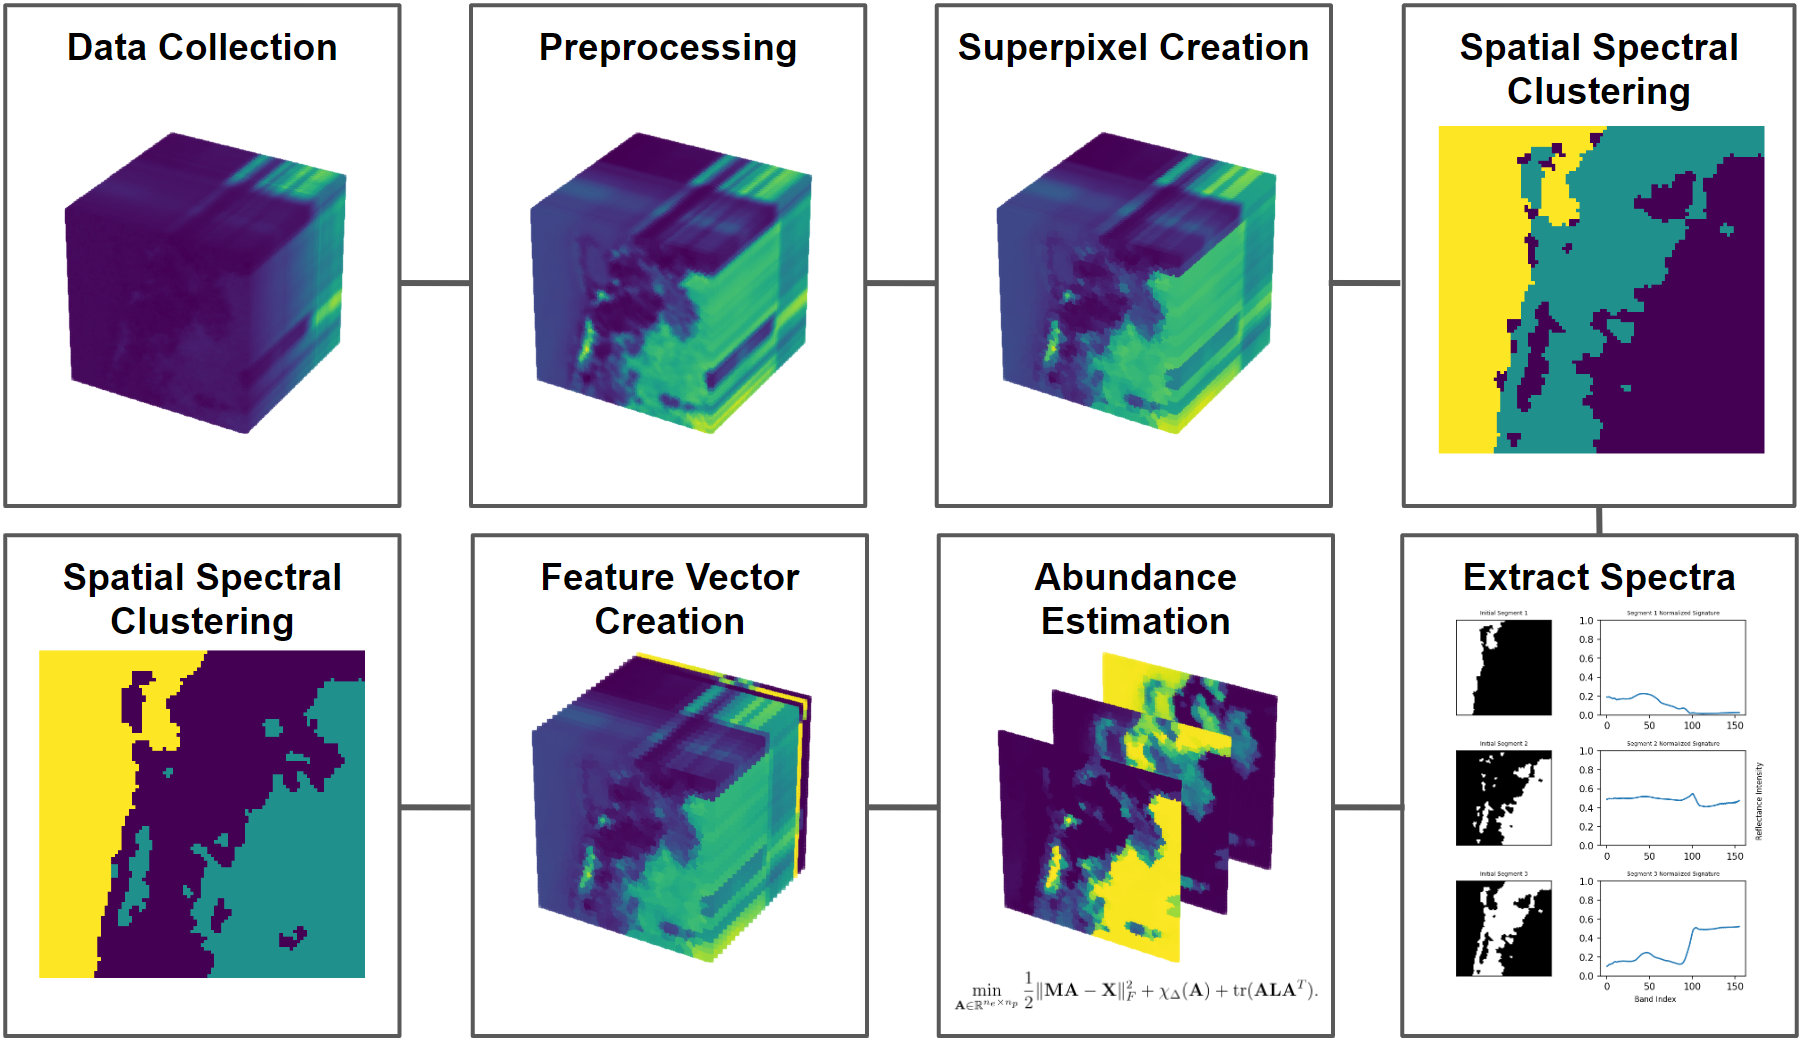
\includegraphics[scale=0.4]{algorithm_view.png}  % Replace filename with your image file name (without extension)
    \label{fig:label}  % Optional label for referencing the figure in the text
  \end{figure}
  

% Current methods for [task] often rely on [existing approach] but suffer from limitations like [limitation 1] and [limitation 2]. To address these challenges, we propose the [Name of your algorithm] algorithm. This algorithm leverages [core idea] to achieve [potential benefit]. We will detail the algorithm's inner workings and evaluate its performance in the following sections.

\clearpage
% \subsection{Proposed Algorithm} \label{Algorithm Overview}
\subsection{Dataset Preprocessing} \label{Algorithm Preprocessing}
As mentioned in Section \ref{Cube}, the input to the algorithm is a hyperspectral image represented by a nonegative tensor $\mathbf{X} \in \mathbb{R}_+^{n_x \times n_y \times n_\lambda}$. Raw hyperspectral images are susceptible to outliers and scale invariance across wavelengths. As such, to ensure algorithms perform reliably along a wide range of domains, preprocessing is a crucial step. Typically, the first main goal of practioners is to deal with noise and regularization across the spectral dimension, then work to deal with spatial artifacts in the image. 
Hyperspectral images often have bands with significantly higher intensity values compared to others. It is important to consider the full collection of wavelengths rather than allow the overprioritization of higher intensity wavelengths, especially in situations where direct scale comparison is made between pixels. By normalizing each spectral band to a similar scale, all spectral bands contribute more equally to the segmentation process. This ensures that results capture the underlying spectral information more effectively. A common approach to normalization in hyperspectral images is band normalization, where intesity values for the hyperspectral image at spectral band $k$, denoted $\mathbf{X}_{(\cdot, \cdot, k)}$ are independently scaled to a range $[0,1]$ according to the minimum and maximum values at that band. Formally,
\begin{equation}
    \label{alg:normalization}
    \hat{\mathbf{X}}_{(\cdot, \cdot, k)} =  \frac{\mathbf{X}_{(\cdot, \cdot, k)} - \min\mathbf{X}_{(\cdot, \cdot, k)}}{\max\mathbf{X}_{(\cdot, \cdot, k)} - \min\mathbf{X}_{(\cdot, \cdot, k)}}.
\end{equation}

% $\mathbf{X}$ can be alternatively represented using matrix $\mathbf{X}_f \in \mathbb{R}_+^{(n_p, n_\lambda)}$, where $n_p = n_x n_y$ is the total number of pixels in the image, with each column representing the pixel at index $(i,j)$ in $\mathbf{X}$, arranged across the first spectral dimension, then the second. Formally, $
% \mathbf{X}_f = \left[ \mathbf{x}_{(0,0)},  \cdots, \mathbf{x}_{(n_x,0)}, \cdots, \mathbf{x}_{(0,n_y)}, \cdots, \mathbf{x}_{(n_x, n_y)} \right] $. 


\subsubsection{Singular Value Decomposition} \label{SVD}
$\mathbf{X}$ can be alternatively represented using a nonnegative matrix $\mathbf{X}_f$ of shape ${(n_\lambda, n_p)}$, where $n_p = n_x n_y$ is the total number of pixels in the image, with each column representing the pixel at index $(i,j)$ in $\mathbf{X}$, arranged across the first spectral dimension, then the second:  $ \mathbf{X}_f = \left[ \mathbf{x}_{(0,0)},  \cdots, \mathbf{x}_{(n_x,0)}, \cdots, \mathbf{x}_{(0,n_y)}, \cdots, \mathbf{x}_{(n_x, n_y)} \right]$. 

do i even need this to be honest?


\subsubsection{Layer Normalization} \label{Normalization}
Hyperspectral images often have bands with significantly higher intensity values compared to others. It is important to consider the full range of wavelengths rather than allow the overprioritization of higher intensity wavelengths, especially in situations where direct scale comparison is made between pixels. By normalizing each spectral band to a similar scale, all spectral bands contribute more equally to the segmentation process. This ensures that results capture the underlying spectral information more effectively. 

A common approach to normalization in hyperspectral images is band normalization, where intesity values for the hyperspectral image at spectral band $k$, denoted $\mathbf{X}_{(\cdot, \cdot, k)}$ are independently scaled to $[0,1]$ according to the minimum and maximum values at that band. Formally,
\begin{equation}
    \label{alg:normalization}
    \hat{\mathbf{X}}_{(\cdot, \cdot, k)} =  \frac{\mathbf{X}_{(\cdot, \cdot, k)} - \min\mathbf{X}_{(\cdot, \cdot, k)}}{\max\mathbf{X}_{(\cdot, \cdot, k)} - \min\mathbf{X}_{(\cdot, \cdot, k)}}.
\end{equation}

\clearpage
% The follow algorithm is proposed

\begin{figure}[h]
    \centering % This centers the image
    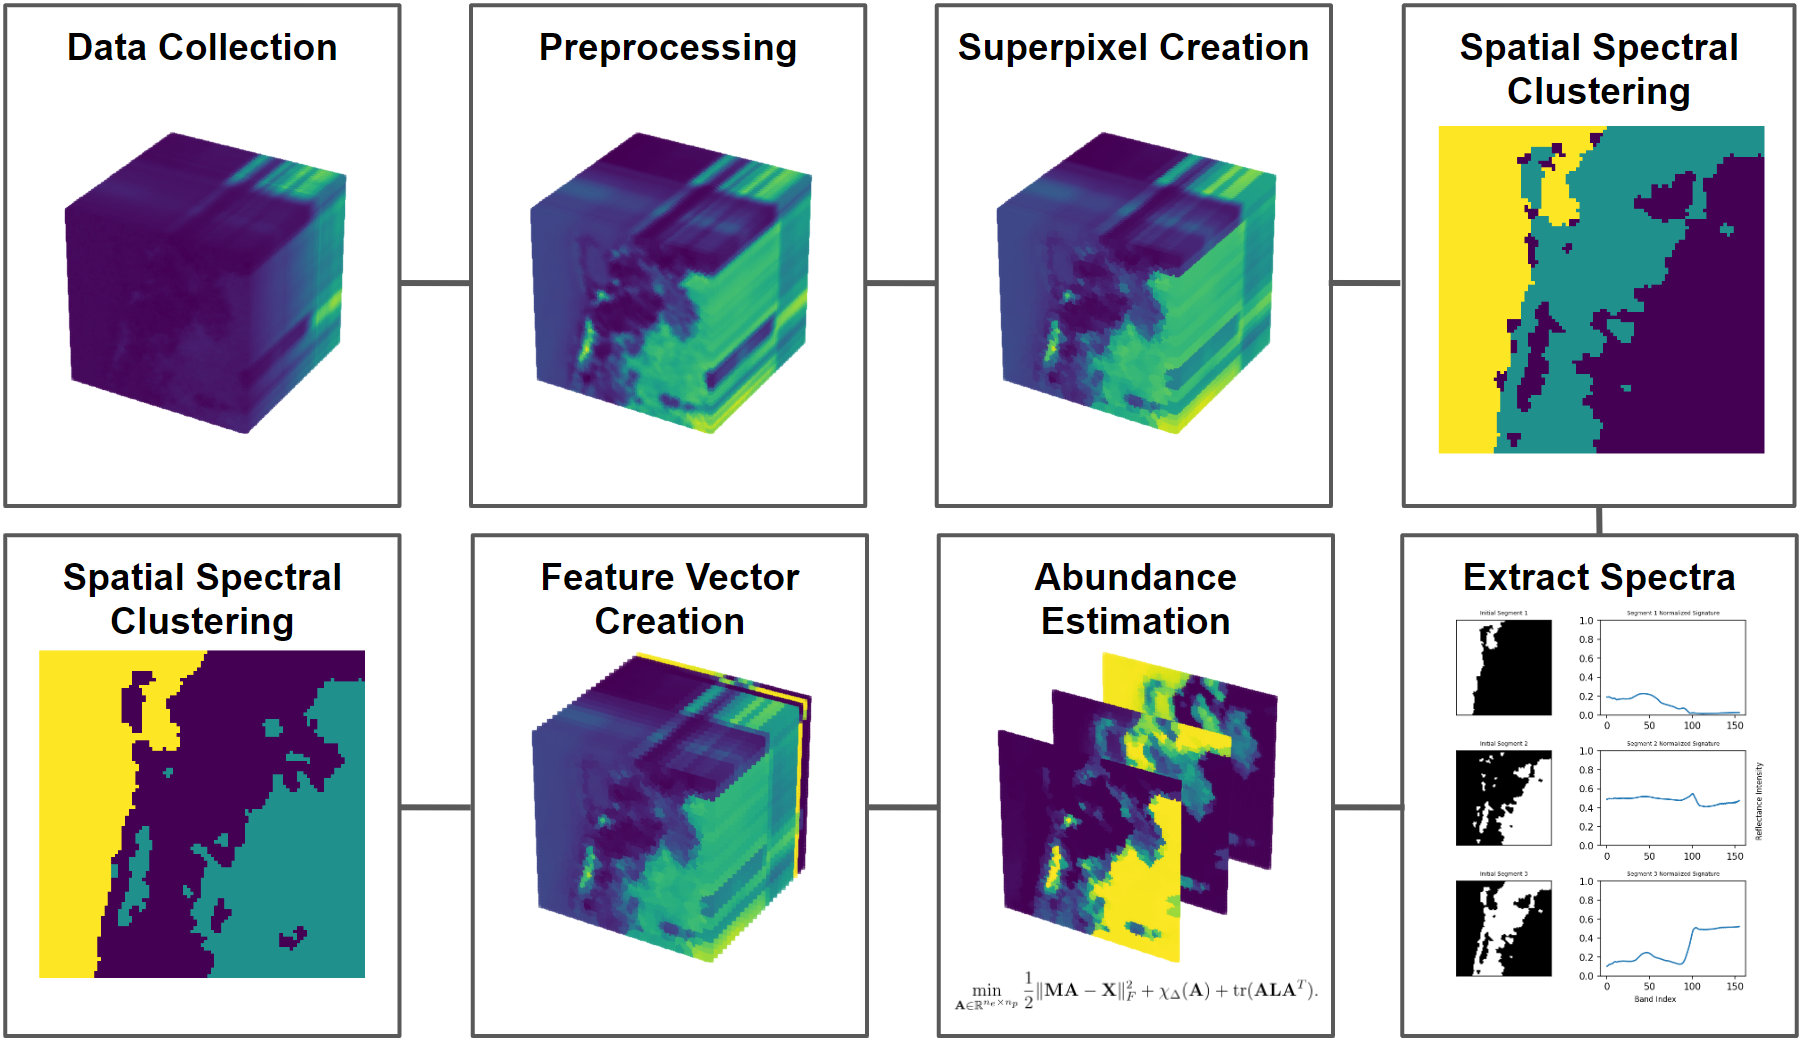
\includegraphics[scale=0.33]{algorithm_view.png}  % Replace filename with your image file name (without extension)
    \label{fig:label}  % Optional label for referencing the figure in the text
  \end{figure}
  
\subsection{Hyperspectral Superpixel Generation} \label{Algorithm Superpixels}
In \ref{SLIC}, the SLIC algorithm was introduced, aiming to perceptually group pixels into locally homogeneous groups called superpixels. While the SLIC algorithm was originally developed for use in the CIELAB colorspace, a similar methodology can be applied towards the hyperspectral space. The main change when trasitioning to the hyperspectral domain requires the consideration of all the spectral features.

With the preprocessed hyperspectral image $\hat{\mathbf{X}}$, each pixel is represented by the vector $\hat{\mathbf{x}}_{(i,j)} = [\hat{x}_1, \hat{x}_2, \dots, \hat{x}_{n_\lambda}]$. Then, taking as an input the number of superpixels $n_s$, superpixel centroids $\mathbf{c}_n = [c_1, c_2, \dots, c_{n_\lambda}]$ where $n = 1,\dots, n_s$ are created at regular grid intervals $S = \sqrt{n_s/n_p}$ across the image. The initial centroids are moved to the lowest gradient position in a $3 \times 3$ spatial neighborhood where the image gradient is now calculated using the original hyperspectral features instead of the CIELAB features: 
\begin{equation}
    \label{eq:slic-gradient-2}
    \mathbb{G}(i,j) = \|\hat{\mathbf{x}}_{(i+1,j)} - \hat{\mathbf{x}}_{(i-1,j)} \|_2^2 + \|\hat{\mathbf{x}}_{(i,j+1)} - \hat{\mathbf{x}}_{(i,j-1)} \|_2^2
\end{equation}

Following the original formulation of the SLIC algorithm, a modified distance measure is proposed to enforce color similarity and spatial extent within the superpixels. Using the same parameter $m$ to control the compactness and shape of the superpixels, the modified distance between a pixel $\hat{\mathbf{x}}$ and cluster $\mathbf{c}_n$ is now calculated as $L_2$ difference between the spectral features plus a scaled version of the spatial euclidean distance between the pixel and the cluster center:
\begin{equation}
    \label{eq:slic-cielab-distance-hsi}
    \mathbb{D}(\hat{\mathbf{x}}, \mathbf{c}_n) = \|\hat{\mathbf{x}} - \mathbf{c}_n\|_2^2 + \frac{m}{S}d_{\text{spatial}}(\hat{\mathbf{x}}, \mathbf{c}_n)^2
\end{equation}

Each pixel is associated with the nearest cluster $\mathbf{c}_n$ whose search area overlaps the pixel. After all pixels are associated with a cluster, a new cluster center is computed as the average vector of all the pixels belonging to the cluster. This is repeated for a set number of iterations. In the hyperspectral version of the SLIC algorithm, the option of relabelling disjoint segments is not performed, instead opting for higher selection of the $m$ and $n_s$ parameters to avoid disjoint segments all together. Once the algorithm is completed, the final superpixeled image is given by arranging the feature vectors into columns of the matrix $\mathbf{C} = [\mathbf{c}_1 \; | \;\mathbf{c}_2 \;| \;\dots \;|\; \mathbf{c}_{n_s}] \in \mathbb{R}^{n_\lambda \times n_s}$. 

\begin{algorithm}[H]
    \label{HSI SLIC}
    \caption{Hyperspectral SLIC Algorithm}
    \textbf{Input}:\\
    \quad  Preprocessed Hyperspectral Image $\hat{\mathbf{X}}$\\
    \quad $m > 0$, $n_s > 0$, $k_{\text{max}}$\\

    \textbf{Initialize:} $\mathbf{c}_n = [c_1, c_2, \cdots, c_{n_\lambda}]$ where $n = 1, \cdots, n_s$ by sampling pixels at regular grid intervals $S$. Perturb cluster centers to lowest gradient position in a $3 \times 3$ neighborhood according to \eqref{eq:slic-gradient-2}. \\
    
    \For{$k = 1$ \KwTo $k_{\text{max}}$}{ 
        Assign best matching pixels from a $2S \times 2S$ neighborhood around clusters $\mathbf{c}_k$ according to \eqref{eq:slic-cielab-distance-hsi}.\\
         Compute new cluster centers according to average of all pixels belonging to cluster.
    }
    \textbf{Output}: Superpixeled Image Matrix $\mathbf{C}$
\end{algorithm}


In the hyperspectral domain, superpixels are slightly less adept at creating visually meaningful partitionings due to use of the raw hyperspectral spectra rather than a perceptual colorspace like CIELAB. To alleviate this, higher values of $m$ and $n_s$ are used to form more spatially compact regions akin to the ones formed in the original algorithm. Nonetheless, superpixels are valuable in allowing practioners to avoid having to consider the variation between individual pixels and instead consider the spectral and spatial variations between these new perceptual groupings of pixels. 

\clearpage
\subsection{Spatial Spectral Clustering}\label{Algorithm Laplacian}
In Section \ref{Spectral Clustering}, the Normalized Cuts algorithm was introduced for the task of bipartitioning a group of pixels through creating an affinity matrix and solving the relaxed eigensystem in \eqref{sc:ncuts-formula}. Considering a matrix of superpixels $\mathbf{C}$ from the results of the SLIC algorithm in Section \ref{Algorithm Superpixels}, two matrices are formed. The first matrix is the spectral affinity matrix $\mathbf{W_{\text{spectral}}}$ given by calculating the spectral angle [REF] between the spectral features of each pair of superpixels:
\begin{equation}
    \label{nc:spectral-mtx}
    \mathbf{W_{\text{spectral}}}_{(i,j)} = \arccos\left(\frac{\mathbf{c}_i \mathbf{c}_j^T}{\|\mathbf{c}_i\|_2\|\mathbf{c}_j\|_2}\right).
\end{equation}
The second matrix is the spatial distance matrix $\mathbf{W_{\text{spatial}}}$ given by calculating the spatial euclidean distance between each pair of superpixels:
\begin{equation}
    \label{nc:spatial-mtx}
    \mathbf{W_{\text{spatial}}}_{(i,j)} = d_{\text{spatial}}(\mathbf{c}_i, \mathbf{c}_j).
\end{equation}
To combine the spatial and spectral information within the image, a spectral similarity parameter $\sigma > 0$ and spatial limit parameter $\kappa > 0$ are introduced and the spatial-spectral affinity matrix $\mathbf{W}$ is then constrcuted as follows
\begin{equation}
    \label{nc:spatial-spectral-mtx}
    \mathbf{W}_{(i,j)} = \begin{cases}
        \exp\left(-\frac{\mathbf{W_{\text{spectral}}}_{(i,j)}^2}{\sigma^2}\right) &\quad \text{if } \mathbf{W_{\text{spatial}}}_{(i,j)} \leq \kappa\\
        0 &\quad \text{if } \mathbf{W_{\text{spatial}}}_{(i,j)} > \kappa.
    \end{cases}
\end{equation}
The intuiton behind constructing the spatial-spectral affinity matrix is to calculate spectral similarity between two superpixels if and only if the centroids of the superpixels are within a spatial range $\kappa$ of each other. This introduces spatial compactness within the partitioning.

After constructing the spatial-spectral affinity matrix, the goal is to to then utilize the normalized cuts algorithm to recursively bipartition the graph $G_\mathbf{W}$ represented by $\mathbf{W}$ into $n_e$ subgraphs. Doing so provides a segmentation of the columns of $\mathbf{C}$ representing the superpixels into $n_e$ clusters. Using the spatial-spectral affinity matrix $\mathbf{W}$, the diagonal matrix $\mathbf{D}$ is calculated according \eqref{sc:d-mtx} and the initial bipartitioning of $G_\mathbf{W}$ can be determined by solving for the second smallest eigenvalue $\lambda_2$ and the corresponding eigenvector $\mathbf{u}_2$ in the system given in \eqref{sc:ncuts-formula}. Bipartitioning the graph $G_\mathbf{W}$ according the sign of the entries in $\mathbf{u}_2$, the next partition is given by the one that minimizes \eqref{sc:ncut-criteria} within the two subgraphs. This process is continued until the graph $G_\mathbf{W}$ is partitioned into $n_e$ subgraphs. Cluster membership of the superpixels in $\mathbf{C}$ are assigned to the corresponding subgraph they belong to. Additionally, the mean spectral signatures of the superpixels within each cluster are calculated and arranged into the matrix $\mathbf{M}$.

\begin{algorithm}[H]
    \label{Spatial Spectral Segmentation}
    \caption{Spatial Spectral Segmentation}
    \textbf{Input}: Superpixel Matrix $\mathbf{C}$, $\kappa > 0$, $\sigma > 0$, $n_e \geq 2$.

    \textbf{Initialize:} Construct the spatial-spectral affinity matrix $\mathbf{W}$ and diagonal matrix $\mathbf{D}$ according to \eqref{nc:spatial-spectral-mtx} and \eqref{sc:d-mtx}.\\

    \textbf{Recursion:}\\
        \quad For each subgraph, solve the system \eqref{sc:ncuts-formula}. Bipartition the subgraph by assigning parition membership according to the cut that minimizes \eqref{sc:ncut-criteria}. 
    \\

    \textbf{Output}: Assign superpixel cluster memberships to a vector $\mathbf{v}_i \in \{1, 2, \dots ,n_e\}$ according to the subgraph each node belongs to. Form a endmember spectra matrix $\mathbf{M} = [ \mathbf{m}_1 | \mathbf{m}_2, | \dots | \mathbf{m}_{n_e} ]$ where $\mathbf{m}_i$ is the average spectral feature vector for all superpixels within the cluster $i$.
\end{algorithm}

The algorithm allows for a flexible and efficient framework for segmentation tasks. The initial construction of the affinity matrix according to \eqref{nc:spatial-spectral-mtx} needs to only be done once, with subsequent subsegmentations being done using selected columns and rows corresponding the the subgraphs each node belongs to. The most obvious bottleneck in the algorithm is the step in which the eigensystem is solved, scalling cubically with the number of superpixels $n_s$. The lower the number of superpixels, the faster the algorithm performs. On the other end, the higher the number of superpixels, the slower the algorithm performs. The final result is determined by tuning $\sigma$ and $\kappa$. The lower $\sigma$ is, the more of an emphasis the spectral features have on the final result, while, the lower $\kappa$ is, the more of an emphasis the spatial information has on the final result. Careful selection of the two parameters allows for meaningful results.


\clearpage
\subsection{Graph Regularized Abundance Estimation}\label{Algorithm Unmixing}
% In Section \ref{AE}, the abundance estimation problem for a collection of pixels $\mathbf{X}$ given the endmember spectra matrix $\mathbf{M}$ was known was stated as follows:

\begin{equation*}
    A = \argmin_{A \in \mathbb{R}^{n_e \times n_p}} \frac{1}{2}\|\mathbf{MA} - \mathbf{X}\|_F^2 + \chi_\Delta(\mathbf{A}) + J(\mathbf{A}).
\end{equation*}
The goal of this section is to demonstrate how this problem can be equivalently represented in a form where the alternating direction method of multipliers technique can be applied. The abundance estimation problem when one or more than one regularization terms are added belongs to a class of problems called global consensus optimization problems shown in Boyd et al. [REF]

Operating under the assumption that $J$ is a convex function, since for nonconvex choices of $J$, convergence is not guarenteed. The approach to transforming \eqref{ae:ae-min-1} is to first introduce matrices $\mathbf{U} \in \mathbb{R}^{n_e \times n_p}$, $\mathbf{V}_1 \in \mathbb{R}^{n_b \times n_p}$, $\mathbf{V}_2 \in \mathbb{R}^{n_e \times n_p}$, and $\mathbf{V}_{3} \in \mathbb{R}^{n_e \times n_p}$ and rewrite as follows:
\begin{equation}
    \label{ae:equivalent-admm-1}
    \begin{aligned}
        \underset{\mathbf{U}, \mathbf{V}_1, \mathbf{V}_2, \mathbf{V}_3}{\text{minimize }} & \quad \frac{1}{2} \|\mathbf{V}_1 - X \|_F^2 + \chi_{\Delta}(\mathbf{V}_2) + J(\mathbf{V}_3) 
        \\         
        \text{subject to } &  \quad \mathbf{V}_1 = \mathbf{MU} \\
        & \quad \mathbf{V}_2 = \mathbf{U} \\
        & \quad \mathbf{V}_{3} = \mathbf{U}
   \end{aligned}
\end{equation}
where
$$g(\mathbf{V}) = \frac{1}{2} \|\mathbf{V}_1 - X \|_F^2 + \chi_{\Delta}(\mathbf{V}_2) + J(\mathbf{V}_3)$$
$$
\mathbf{V} = \begin{bmatrix}
\mathbf{V}_1 &  &   \\
 &\mathbf{V}_2&   \\
  &  & \mathbf{V}_3 \\
\end{bmatrix},
\quad
\mathbf{G} = 
\begin{bmatrix}
\mathbf{M}\\ 
\mathbf{I}\\ 
\mathbf{I}\\ 
\end{bmatrix},
\quad
\mathbf{B} = 
\begin{bmatrix}
-\mathbf{I} &  &  \\
  &-\mathbf{I}&  \\
&  & -\mathbf{I} \\
\end{bmatrix}.
$$
The problem depicted in \eqref{ae:equivalent-admm-1} can then be rewritten in equivalent form:
\begin{equation}
    \label{ae:equivalent-admm-2}
    \begin{aligned}
        \underset{\mathbf{U},\mathbf{V}}{\text{minimize }} & \quad g(\mathbf{V})
        \\         
        \text{subject to } &  \quad \mathbf{GU} + \mathbf{BV} = \mathbf{0}
   \end{aligned}
\end{equation}
The scaled augmented lagrangian $\mathcal{L}_\mu$ with parameter $\mu > 0$ and scaled dual variable $\mathbf{D}$ is then given as:
\begin{equation}
  \label{admm:lagrangian-ae}
  \mathcal{L}_{\mu}(\mathbf{U}, \mathbf{V}, \mathbf{D}) = g(\mathbf{V}) + \frac{\mu}{2} \|\mathbf{GU} + \mathbf{BV} - \mathbf{D}\|_F^2
\end{equation}
where
$$
\mathbf{D} = 
\begin{bmatrix}
\mathbf{D}_1 &  &  \\
  &\mathbf{D}_2&  \\
&  & \mathbf{D}_3 \\
\end{bmatrix}.
$$
ADMM aims to minimize scaled form of $\mathcal{L}_{\mu}$ by alternating minimizations with respect to $\mathbf{U}$, $\mathbf{V}$, and $\mathbf{D}$ by performing the following updates:
\begin{equation}
  \label{admm:ae-updates}
  \begin{aligned}
    \mathbf{U}^{(k+1)} &= \argmin_{\mathbf{U}}  \frac{\mu}{2} \|\mathbf{GU} + \mathbf{BV}^{(k)} - \mathbf{D}^{(k)}\|_F^2 \\
    \mathbf{V}^{(k+1)} &= \argmin_{\mathbf{V}} g(\mathbf{V}) + \frac{\mu}{2} \|\mathbf{GU}^{(k+1)} + \mathbf{BV} - \mathbf{D}^{(k)}\|_F^2 \\
    \mathbf{D}^{(k+1)} &= \mathbf{D}^{(k)} - \mathbf{GU}^{(k+1)} - \mathbf{BV}^{(k+1)}.
    \end{aligned}
\end{equation}

While the updates are in a simpler format, further work needs to be done to derive updates for $\mathbf{V}$. Looking at the $\|\mathbf{GU} + \mathbf{BV}^{(k)} - \mathbf{D}^{(k)}\|_F^2$ term in \eqref{admm:lagrangian-ae}, the structure of it's components give leeway to splitting the term into individual components, notably
\begin{equation*}
  \begin{aligned}
    \|\mathbf{GU} + \mathbf{BV} - \mathbf{D}\|_F^2 &= 
    \left\lVert
    \begin{bmatrix}
    \mathbf{MU} - \mathbf{V}_1 - \mathbf{D}_1 &  &  \\
      &\mathbf{U} - \mathbf{V}_2 - \mathbf{D}_2&  \\
    &  & \mathbf{U} - \mathbf{V}_3 - \mathbf{D}_3 \\
    \end{bmatrix}
    \right\rVert^2_F \\
    &= \|\mathbf{MU} - \mathbf{V}_1 - \mathbf{D}_1\|_F^2 +
       \|\mathbf{U} - \mathbf{V}_2 - \mathbf{D}_2\|_F^2 +
       \|\mathbf{U} - \mathbf{V}_3 - \mathbf{D}_3\|_F^2.
  \end{aligned}
\end{equation*}
Applying this expansion, the updates in \eqref{admm:ae-updates} can be rewritten. The $\mathbf{U}$ update becomes
\begin{equation}
  \label{admm:ae-updates-u}
  \begin{aligned}
    \mathbf{U}^{(k+1)} = \argmin_{\mathbf{U}}  & 
    \frac{\mu}{2} \|\mathbf{MU} - \mathbf{V}_1^{(k)} - \mathbf{D}_1^{(k)}\|_F^2 \\
    & + \frac{\mu}{2} \|\mathbf{U} - \mathbf{V}_2^{(k)} - \mathbf{D}_2^{(k)}\|_F^2 \\
    & + \frac{\mu}{2} \|\mathbf{U} - \mathbf{V}_3^{(k)} - \mathbf{D}_3^{(k)}\|_F^2.
  \end{aligned}
\end{equation}
Under the same expansion, the $\mathbf{V}$ update becomes
\begin{equation*}
  \begin{aligned}
    \mathbf{V}^{(k+1)} = \argmin_{\mathbf{V}}  &  \frac{1}{2} \|\mathbf{V}_1 - X \|_F^2 + \chi_{\Delta}(\mathbf{V}_2) + J(\mathbf{V}_3) \\ 
    & + \frac{\mu}{2} \|\mathbf{MU}^{(k+1)} - \mathbf{V}_1 - \mathbf{D}_1^{(k)}\|_F^2 \\
    & + \frac{\mu}{2} \|\mathbf{U}^{(k+1)} - \mathbf{V}_2 - \mathbf{D}_2^{(k)}\|_F^2 \\
    & + \frac{\mu}{2} \|\mathbf{U}^{(k+1)} - \mathbf{V}_3 - \mathbf{D}_3^{(k)}\|_F^2.
  \end{aligned}
\end{equation*}
Furthermore, each component of the update for $\mathbf{V}$ can be split into individual updates for $\mathbf{V}_1$, $\mathbf{V}_2$ and $\mathbf{V}_3$:
\begin{equation}
  \label{admm:ae-updates-v}
  \begin{aligned}
    \mathbf{V}_1^{(k+1)} &= \argmin_{\mathbf{V}_1} \frac{1}{2} \|\mathbf{V}_1 - X \|_F^2 + \frac{\mu}{2} \|\mathbf{MU}^{(k+1)} - \mathbf{V}_1 - \mathbf{D}_1^{(k)}\|_F^2 \\
    \mathbf{V}_2^{(k+1)} &= \argmin_{\mathbf{V}_2} \chi_{\Delta}(\mathbf{V}_2) + \frac{\mu}{2} \|\mathbf{U}^{(k+1)} - \mathbf{V}_2 - \mathbf{D}_2^{(k)}\|_F^2 \\
    \mathbf{V}_3^{(k+1)} &= \argmin_{\mathbf{V}_3} J(\mathbf{V}_3) + \frac{\mu}{2} \|\mathbf{U}^{(k+1)} - \mathbf{V}_3 - \mathbf{D}_3^{(k)}\|_F^2
  \end{aligned}
\end{equation}
Lastly, in similar fashion to $\mathbf{V}$, the $\mathbf{D}$ update in \eqref{admm:ae-updates} can also be split component wise:
\begin{equation}
  \label{admm:ae-updates-d}
  \begin{aligned}
    \mathbf{D}_1^{(k+1)} &= \mathbf{D}_1^{(k)} - \mathbf{MU}^{(k+1)} + \mathbf{V}_1^{(k+1)} \\
    \mathbf{D}_2^{(k+1)} &= \mathbf{D}_2^{(k)} - \mathbf{U}^{(k+1)} + \mathbf{V}_2^{(k+1)} \\
    \mathbf{D}_3^{(k+1)} &= \mathbf{D}_3^{(k)} - \mathbf{U}^{(k+1)} + \mathbf{V}_3^{(k+1)}.
  \end{aligned}
\end{equation}
Taking into account \eqref{admm:ae-updates-u}, \eqref{admm:ae-updates-v}, \eqref{admm:ae-updates-d}, the updates in \eqref{admm:ae-updates} can finally be rewritten in the expanded form as:
\begin{equation}
  \label{admm:ae-updates-final}
  \begin{aligned}
    \mathbf{U}^{(k+1)} & = \argmin_{\mathbf{U}}  
    \frac{\mu}{2} \|\mathbf{MU} - \mathbf{V}_1^{(k)} - \mathbf{D}_1^{(k)}\|_F^2  + \frac{\mu}{2} \|\mathbf{U} - \mathbf{V}_2^{(k)} - \mathbf{D}_2^{(k)}\|_F^2  + \frac{\mu}{2} \|\mathbf{U} - \mathbf{V}_3^{(k)} - \mathbf{D}_3^{(k)}\|_F^2 
    \\
    \mathbf{V}_1^{(k+1)} &= \argmin_{\mathbf{V}_1} \frac{1}{2} \|\mathbf{V}_1 - X \|_F^2 + \frac{\mu}{2} \|\mathbf{MU}^{(k+1)} - \mathbf{V}_1 - \mathbf{D}_1^{(k)}\|_F^2 \\
    \mathbf{V}_2^{(k+1)} &= \argmin_{\mathbf{V}_2} \chi_{\Delta}(\mathbf{V}_2) + \frac{\mu}{2} \|\mathbf{U}^{(k+1)} - \mathbf{V}_2 - \mathbf{D}_2^{(k)}\|_F^2 \\
    \mathbf{V}_3^{(k+1)} &= \argmin_{\mathbf{V}_3} J(\mathbf{V}_3) + \frac{\mu}{2} \|\mathbf{U}^{(k+1)} - \mathbf{V}_3 - \mathbf{D}_3^{(k)}\|_F^2 \\
    \mathbf{D}_1^{(k+1)} &= \mathbf{D}_1^{(k)} - \mathbf{MU}^{(k+1)} + \mathbf{V}_1^{(k+1)} \\
    \mathbf{D}_2^{(k+1)} &= \mathbf{D}_2^{(k)} - \mathbf{U}^{(k+1)} + \mathbf{V}_2^{(k+1)} \\
    \mathbf{D}_3^{(k+1)} &= \mathbf{D}_3^{(k)} - \mathbf{U}^{(k+1)} + \mathbf{V}_3^{(k+1)}.
  \end{aligned}
\end{equation}

The updates for $\mathbf{U}$ and $\mathbf{V}_1$ have closed form solutions due to convexity and differentiability of the Frobenius norm [REF]. Both updates can derived by taking the first partial derivatives with respect to the individual terms, setting it equal to $\mathbf{0}$, and solving accordingly. For the $\mathbf{U}$ update,
$$
  \begin{aligned}
    0 &= \frac{\partial}{\partial \mathbf{U}}\left[\frac{\mu}{2} \|\mathbf{MU} - \mathbf{V}_1 - \mathbf{D}_1\|_F^2  + \frac{\mu}{2} \|\mathbf{U} - \mathbf{V}_2 - \mathbf{D}_2\|_F^2  + \frac{\mu}{2} \|\mathbf{U} - \mathbf{V}_3 - \mathbf{D}_3\|_F^2\right]
    \\
    0 &= \mu \left(\mathbf{M}^T(\mathbf{MU}-\mathbf{V}_1-\mathbf{D}_1) + (\mathbf{U}-\mathbf{V}_2-\mathbf{D}_2) + (\mathbf{U}-\mathbf{V}_3-\mathbf{D}_3)\right)
    \\
    \mathbf{M}^T\mathbf{MU} + 2\mathbf{U} &= \mathbf{M}^T(\mathbf{V}_1+\mathbf{D}_1) + (\mathbf{V}_2+\mathbf{D}_2) + (\mathbf{V}_3+\mathbf{D}_3)
    \\
    \mathbf{U} &= (\mathbf{M}^T \mathbf{M} + 2\mathbf{I})^{-1}(\mathbf{M}^T(\mathbf{V}_1+\mathbf{D}_1) + (\mathbf{V}_2+\mathbf{D}_2) + (\mathbf{V}_3+\mathbf{D}_3)).
  \end{aligned}
$$
As $\mathbf{M}$ is known, $(\mathbf{M}^T \mathbf{M} + 2\mathbf{I})^{-1}$ can be calculated once for the entire program. For the $\mathbf{V}$ update,
$$
\begin{aligned}
  0 &= \frac{\partial}{\partial \mathbf{V}_1} \left[ \frac{1}{2}\|\mathbf{V}_1-\mathbf{X}\|_F^2 + \frac{\mu}{2} \|\mathbf{MU} - \mathbf{V}_1 - \mathbf{D}_1 \|_F^2 \right]
  \\
  0 &= (\mathbf{V}_1 - \mathbf{X}) + \mu(\mathbf{V}_1 - (\mathbf{MU} - \mathbf{D}_1))
  \\
  \mathbf{V}_1 &= \frac{1}{1+\mu} \left(\mathbf{X} + (\mathbf{MU} - \mathbf{D}_1)\right).
\end{aligned}
% 0 &= \frac{\partial}{\partial V_1} \left[ \frac{1}{2}\|V_1-X\|_F^2 + \frac{\tau}{2} \|MU - V_1 - D_1 \|_F^2 \right] \\
% 0 &= (V_1 - X) + \tau(V_1 - (MU - D_1)) \\
% V_1 &= \frac{1}{1+\tau} \left(X + (MU - D_1)\right)
% \end{aligned}
$$
% While the update for $\mathbf{V}_2$ does not have a closed form solution, the convexity of $\Delta$ allows for the use of an alternating projection based method for finding an approximate solution to the update. $\Delta$ itself is the intersection of two convex sets $\mathbb{R}^{n_e \times n_p}_+$ and $\{ \mathbf{A} \in \mathbb{R}^{n_e \times n_p} \mid \mathbf{1}_{n_e}^T \mathbf{A} = \mathbf{1}_{n_p}\}$. It is important to note that the update $\mathbf{V}_2$ can be rewritten as 

While the update for $\mathbf{V}_2$ does not have a closed form solution, it is important to note that the update $\mathbf{V}_2$ can be equivalently rewritten as:
$$
\mathbf{V}_2^{(k+1)} = \argmin_{\mathbf{V}_2 \in \Delta} \frac{\mu}{2} \|\mathbf{U}^{(k+1)} - \mathbf{V}_2 - \mathbf{D}_2^{(k)}\|_F^2.
$$
The update, in non-formulaic terms, requires finding $\mathbf{V}_2$ that minimizes $\frac{\mu}{2} \|\mathbf{U}^{(k+1)} - \mathbf{V}_2 - \mathbf{D}_2^{(k)}\|_F^2$, then projecting the solution onto $\Delta$. 
The non-projected minimum can be found in the same way as the updates for $\mathbf{V}$ and $\mathbf{U}$
\begin{equation*}
  \begin{aligned}
    0 &= \frac{\partial}{\partial \mathbf{V}_2} \left[\frac{\mu}{2} \|\mathbf{U} - \mathbf{V}_2 - \mathbf{D}_2\|_F^2\right]
    \\
    0 &= \mu(\mathbf{V}_2 - (\mathbf{MU} - \mathbf{D}_2))
    \\
    \mathbf{V}_2 &= \mathbf{MU} - \mathbf{D}_2
  \end{aligned}
\end{equation*}
The orthogonal projection of a matrix $\mathbf{X}$ onto $\Delta$ is defined as the finding the matrix $\tilde{\mathbf{X}} \in \Delta$ that minimizes the least-squares error between the two matrices. The convexity of $\Delta$ and the additional property that $\Delta$ is closed ensures that the projection is unique. Multiple numerical methods exist for computing the projection [REF]. Formally,
\begin{equation*}
  \text{proj}_\Delta(\mathbf{X}) = \argmin_{\tilde{\mathbf{X}} \in \Delta} \|\tilde{\mathbf{X}} - \mathbf{X}\|_F^2.
\end{equation*}
Thus, applying the projection, the update for $\mathbf{V}_2$ is given as
\begin{equation*}
  \mathbf{V}_2 = \text{proj}_\Delta(\mathbf{MU} - \mathbf{D}_2).
\end{equation*}

After deriving solutions for $\mathbf{V}_1$, $\mathbf{V}_2$, $\mathbf{U}$, the updates in \eqref{admm:ae-updates} can be written as:
\begin{equation}
  \label{admm:ae-updates-final-2}
  \begin{aligned}
    \mathbf{U}^{(k+1)} & = (\mathbf{M}^T \mathbf{M} + 2\mathbf{I})^{-1}(\mathbf{M}^T(\mathbf{V}_1^{(k)}+\mathbf{D}_1^{(k)}) + (\mathbf{V}_2^{(k)}+\mathbf{D}_2^{(k)}) + (\mathbf{V}_3^{(k)}+\mathbf{D}_3^{(k)})).
    \\
    \mathbf{V}_1^{(k+1)} &= \frac{1}{1+\mu} \left(\mathbf{X} + (\mathbf{MU}^{(k+1)} - \mathbf{D}_1^{(k)})\right) 
    \\
    \mathbf{V}_2^{(k+1)} &= \text{proj}_\Delta(\mathbf{MU}^{(k+1)} - \mathbf{D}_2^{(k)}) 
    \\
    \mathbf{V}_3^{(k+1)} &= \argmin_{\mathbf{V}_3} J(\mathbf{V}_3) + \frac{\mu}{2} \|\mathbf{U}^{(k+1)} - \mathbf{V}_3 - \mathbf{D}_3^{(k)}\|_F^2 
    \\
    \mathbf{D}_1^{(k+1)} &= \mathbf{D}_1^{(k)} - \mathbf{MU}^{(k+1)} + \mathbf{V}_1^{(k+1)} 
    \\
    \mathbf{D}_2^{(k+1)} &= \mathbf{D}_2^{(k)} - \mathbf{U}^{(k+1)} + \mathbf{V}_2^{(k+1)} 
    \\
    \mathbf{D}_3^{(k+1)} &= \mathbf{D}_3^{(k)} - \mathbf{U}^{(k+1)} + \mathbf{V}_3^{(k+1)}.
  \end{aligned}
\end{equation}

Leaving the update for $\mathbf{V_3}$ as the only minimization problem for practicioners to derive the update for. Many variations of the abundance estimation problem exist where one or more regularization terms on $\mathbf{A}$ are added for further control over the final solution. This technique can be further extended to consider $m$ regularization terms $J_1, \dots, J_m$, in which the result is $m+2$ additional updates for the subproblems arising from splitting $\mathbf{V}$ and $m+2$ additional updates for the subproblems arising from splitting $\mathbf{D}$. The alternating direction method of multipliers technique is most useful in situations where multiple regularization terms exist in the loss function and no closed form solution exist, demonstrating it's superiority in the field of hyperspectral image analysis.
\subsection{Feature Vector Creation}\label{Algorithm FV}
The abundance estimation problem described in Section \ref{Algorithm Unmixing} outputs a matrix $ \mathbf{A} \in \mathbb{R}_+^{n_e \times n_p}$ whose columns $\mathbf{a}_i$ hold the abundance values for the superpixel $\mathbf{c}_i$ with respect to the mean spectral signatures. The initial partitioning of the set of superpixels performed in Section \ref{Algorithm NCuts} often provides an adequate solution, however, there is always hope to further refine the segmentation (\cite{SSBD}). In the effort to do so, a new superpixel feature vector is created by concatenating the original spectral features and the abundance estimation results
\begin{equation}
    \label{Feature Vector Creation}
    \tilde{\mathbf{c}}_i = \mathbf{c}_i \oplus \mathbf{a}_i
\end{equation}

With the new construction of $\tilde{\mathbf{c}}$, the segmentation described in Section \ref{Algorithm NCuts} is repeated with the same set of parameters $\sigma$ and $\kappa$. The overall intuition behind this final step is to combine these additional, rich abundance features and the original spectral information to produce a more accurate segmentation. This proves useful along the boundaries between regions, where the creation of superpixels leads to mixed pixels. The added abundance information aids in adequately segmenting these mixed regions. The further refinement through the inclusion of the abundance information allows stronger spatial coherence in the clusters, due to the use of the graph regularization in \eqref{unmixing:graph-reg-ae}.


\subsection{Compilation}\label{Compilation}
In summary, the algorithm can be described as follows

\begin{algorithm}[H]
    \caption{Adaptive Superpixel Cuts for Hyperspectral Images}
    \textbf{Input}: \\
    \quad Hyperspectral Image $\mathbf{X} \in \mathbb{R}_+^{n_x \times n_y \times n_\lambda}$. \\
    \quad Superpixel Parameters: $n_s$, $m$\\
    \quad Segmentation Parameters: $n_e$, $\sigma$ , $\kappa$ \\
    \quad Abundance Estimation Parameters: $\mu$ , $\beta$
    \\
    \textbf{Preprocessing:}\\ \quad Create Normalized Hyperspectral Image $\hat{\mathbf{X}}$ according to \eqref{alg:normalization}.
    \\
    \textbf{Superpixel Creation:}\\ \quad Generate superpixel matrix $\mathbf{C} \in \mathbb{R}_+^{n_\lambda \times n_s}$ according to Algorithm \ref{HSI SLIC} with parameters $n_s$, $m$.
    \\
    \textbf{Spatial Spectral Segmentation:}\\ \quad Perform an initial segmentation of the columns of the superpixel matrix $\mathbf{C}$ into $n_e$ partitions and form the spectra matrix $\mathbf{M} \in \mathbf{R}_+^{n_\lambda \times n_e}$ according to Algorithm \ref{Spatial Spectral Segmentation} with parameters $n_e$, $\sigma$, $\kappa$.
    \\
    \textbf{Abundance Estimation:}\\ \quad Perform abundance estimation to the columns of the superpixel matrix $\mathbf{C}$ relative to the spectra matrix $\mathbf{M}$, obtaining abudance matrix $A \in \mathbb{R}_+^{n_e \times n_s} $ according to Algorithm \ref{Graph Regularized AE} with parameters $\mu$ , $\beta$.
    \\
    \textbf{Feature Vector Creation}\\ \quad Form the feature matrix $\tilde{\mathbf{C}} \in \mathbb{R}_+^{(n_\lambda + n_e) \times n_s}$ according to \eqref{Feature Vector Creation}
    \\
    \textbf{Spatial Spectral Segmentation:}\\ \quad Perform the final segmentation of the columns of the superpixel matrix $\tilde{\mathbf{C}}$ into $n_e$ partitions according to Algorithm \ref{Spatial Spectral Segmentation} with parameters $n_e$, $\sigma$, $\kappa$.
    \\
    \textbf{Output}:\\
    \quad Label vector $\mathbf{v}$, where $v_i \in {1,2, \cdots, n_e}$, corresponding to the final segmentation of the superpixels.
  \end{algorithm}

The superpixel parameters $n_s$ and $m$ are one time selections based off the requirements of the practioners, as $n_s$ determines the runtime of the algorithm. If $n_s$ is set too high, the more the superpixels resemble the original image itself, giving zero benefit to using a superpixel approach. Careful and reasonable selection of $n_s$ and $m$ should be done based off the requirements of the specific analysis to be done. In practice, setting $n_s$ such that $\frac{n_p}{n_s} \approx 16$ allows adequate results without extensive tuning of $m$. In similar fashion, the abundance estimation parameters $\mu$ and $\beta$ are one time, global selections. As mentioned in Section \ref{ADMM Intro}, the ADMM method provides modest accuracy solutions in a relatively low number of operations. In practice, the results of the algorithm are largerly insensitive to selection of $\mu$. In a similar manner, $\beta$ serves the purpose of reducing relative variations in abundance estimates between nearby superpixels, which aids in instances where two regions share similar spectral characteristics but are spatially distinct. 

In application, the choice of parameters primarily focuses on on the segmentation parameters $n_e$, $\sigma$ , $\kappa$ as they dictate the initial and final segmentation of the image itself. Selection should be done to ensure an informative intial segmentation, then allow the algorithm to further refine it for the final segmentation according to the specific domain requirements.
\subsection{Parameter Selection}\label{Parameters}


\clearpage
% #############################################
% 
% 
% 
% 
% 
% #############################################
\section{Experimental Results}


\subsection{Implementation Details}

\clearpage
\subsection{Geospatial Testing Datasets}
\subsubsection{Samson Datasets}
\subsubsection{Salinas Datasets}
\subsubsection{Biomedical Autofluorescence Dataset}

\clearpage
\subsection{Algorithm Evaluation}
\subsubsection{Qualitative Evaluation on Samson}
\subsubsection{Quantitative Evaluation on Salinas}
\subsubsection{Qualitative Evaluation on Biomedical Autofluorescence Data}

\clearpage
\subsection{Algorithm Comparison}

\clearpage
% #############################################
% 
% 
% 
% 
% 
% #############################################

\clearpage
% #############################################
% 
% 
% 
% 
% 
% #############################################
\section{Conclusions}

\end{document}